\RequirePackage{luatex85}
\documentclass{standalone}
\usepackage{tikz}
\usetikzlibrary{decorations}
\usetikzlibrary{decorations.pathmorphing}
\usetikzlibrary{arrows.meta}
\tikzset{>=latex, line width=1.0pt}
\usepackage{amsmath}
\usepackage{mathtools}
\newcommand{\ct}{\hspace{2pt}\rule[1pt]{3pt}{3pt}\hspace{2pt}}
\DeclareMathOperator{\pr}{pr}
\DeclareMathOperator{\transport}{transport}
\begin{document}
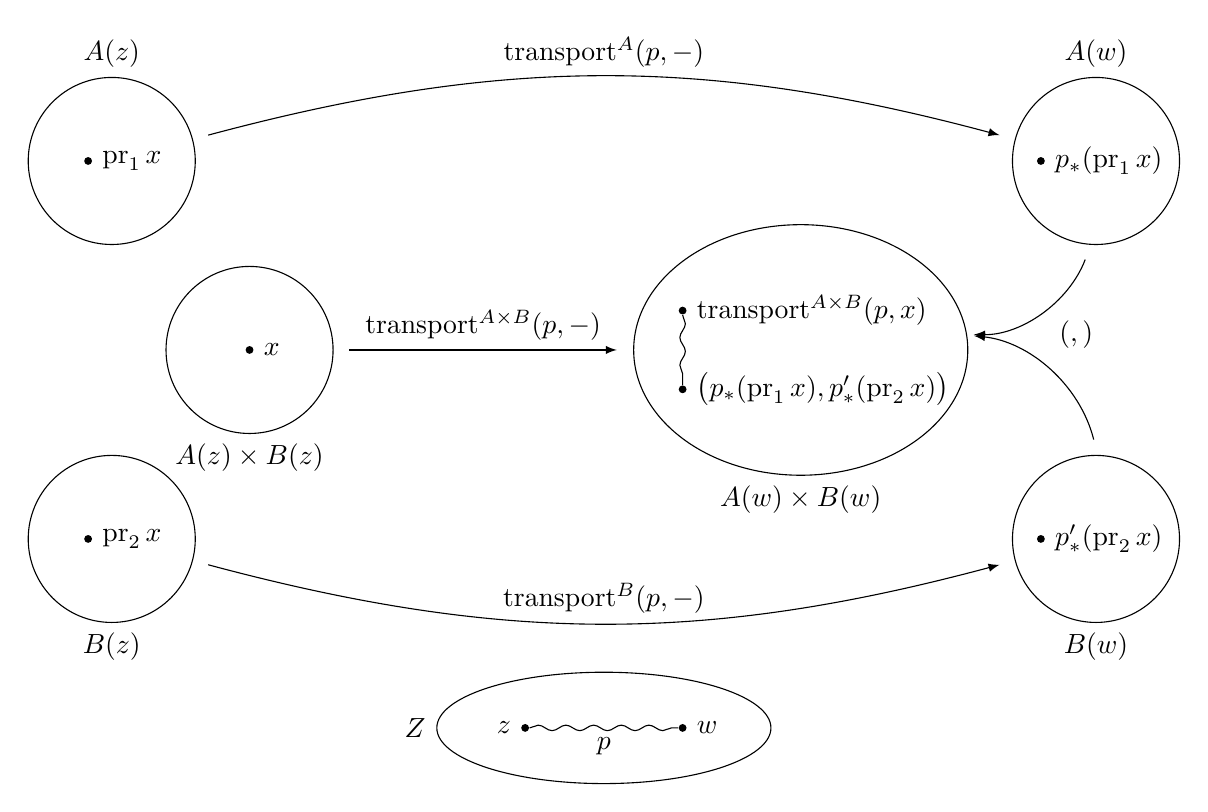
\begin{tikzpicture}
  \def\xshift{2.5}
  \def\yheight{2.4}

  % A(z)
  \node[circle,draw,inner sep=0.75cm,label=above:{$A(z)$}]
    (Az) at (-2.5*\xshift,3*\yheight) {};
  % B (z)
  \node[circle,draw,inner sep=0.75cm,label=below:{$B(z)$}]
    (Bz) at (-2.5*\xshift,1*\yheight) {};
  % A(z) x B(z)
  \node[circle,draw,inner sep=0.75cm,label=below:{$A(z)\times B(z)$}]
    (AzBz) at (-1.8*\xshift,2*\yheight) {};
  \node[circle,fill,inner sep=1pt,label=right:{$x$}] (x) at (AzBz) {};

  % Points
  \node[circle,fill,inner sep=1pt,xshift=-0.3cm,label=right:{$\pr_1x$}]
    (pr1x) at (Az) {};
  \node[circle,fill,inner sep=1pt,xshift=-0.3cm,label=right:{$\pr_2x$}]
    (pr1x) at (Bz) {};

  % A(w)
  \node[circle,draw,inner sep=0.75cm,label=above:{$A(w)$}]
    (Aw) at (2.5*\xshift,3*\yheight) {};
  % B (w)
  \node[circle,draw,inner sep=0.75cm,label=below:{$B(w)$}]
    (Bw) at (2.5*\xshift,1*\yheight) {};
  % A(w) x B(w)
  \node[circle,draw,xscale=2.0,yscale=1.5,inner sep=0.75cm,label=below:{$A(w)\times B(w)$}]
    (AwBw) at (\xshift,2*\yheight) {};

  % Points
  \node[circle,fill,inner sep=1pt,xshift=-0.7cm,label=right:{$p_*(\pr_1x)$}]
    (pr1x) at (Aw) {};
  \node[circle,fill,inner sep=1pt,xshift=-0.7cm,label=right:{$p_*'(\pr_2x)$}]
    (pr1x) at (Bw) {};
  \node[circle,fill,inner sep=1pt,xshift=-1.5cm,yshift=0.5cm,label=right:{$\transport^{A\times B}(p,x)$}] (t1) at (AwBw) {};
  \node[circle,fill,inner sep=1pt,xshift=-1.5cm,yshift=-0.5cm,label=right:{$\big(p_*(\pr_1x),p_*'(\pr_2x)\big)$}] (t2) at (AwBw) {};
  \draw[decorate,decoration={snake,amplitude=1}] (t1) --  (t2);


  % various transports
  \draw[->,shorten >=0.2cm,shorten <=0.2cm] (AzBz) to[]
    node[above] {$\operatorname{transport}^{A\times B}(p,-)$} (AwBw) {};
  \draw[->,shorten >=0.2cm,shorten <=0.2cm] (Az) to[bend left=15]
    node[auto] {$\operatorname{transport}^{A}(p,-)$} (Aw) {};
  \draw[->,shorten >=0.2cm,shorten <=0.2cm] (Bz) to[bend right=15]
    node[auto] {$\operatorname{transport}^{B}(p,-)$} (Bw) {};

  % pairing
  \draw[->,shorten >=0.2cm,shorten <=0.2cm] (Aw) to[bend left=35] (4.5,5) {};
  \draw[->,shorten >=0.2cm,shorten <=0.2cm] (Bw) to[bend right=35] (4.5,5) {};
  \node[] (Bw) at (6,5) {$(,)$};

  % Base space Z
  \node[circle,draw,inner sep=0.5cm,label=left:{$Z$},xscale=3.0,yscale=1.0] (A) at (0,0) {};
  \node[circle,fill,inner sep=1pt,label=left:{$z$}] (z) at (-1.0,0) {};
  \node[circle,fill,inner sep=1pt,label=right:{$w$}] (w) at (1.0,0) {};
  \draw[decorate,decoration={snake,amplitude=1}] (z) -- node[auto,swap] {$p$} (w);
\end{tikzpicture}
\end{document}